\textbf{\large\color{orange}Zadanie 5.} Mapą na powierzchni $M$ nazywamy podział powierzchni na komórki homeomorficzne z dyskami, których przekroje są zawarte w ich brzegach. Z takim podziałem
mamy związany graf dualny, którego wierzchołki, to komórki, a krawędź istnieje
pomiędzy wierzchołkami, gdy odpowiadające im komórki mają niepusty przekrój.
Kolorowaniem mapy nazywać będziemy funkcję ze zbioru komórek w pewien skończony zbiór kolorów, która przyjmuje różne wartości na krojących się niepusto
komórkach.
\begin{enumerate}[label=(\alph*)]
  \item Jak mogą wyglądać mapy na powierzchniach? Czy da się uprościć je tak, by
graf dualny był $1$-szkieletem triangulacji? Rozważyć mapę o sześciu krajach
na butelce Kleina.
\item Twierdzenie o $k$ barwach dla powierzchni $M$ mówi, że każdą mapę na powierzchni $M$ można pokolorować co najwyżej $k$ kolorami. Udowodnić twierdzenie o $5$ barwach dla sfery $S^2$, o $6$ barwach dla $RP^2$ o $7$ barwach dla torusa
$T^2$ i o $6$ barwach dla butelki Kleina.
\end{enumerate}

\dotfill 

\begin{enumerate}[label=\textbf{(\alph*)}]
  \item W mapie pozwalamy, aby w jednym punkcie spotykały się co najwyżej $3$ kraje. Jeśli istnieje punkt, w którym spotykają się $4$ kraje, wtedy ten punkt zamieniamy na krawędź:
    \begin{center}\begin{tikzpicture}
      \fill [pattern={Dots[radius=1pt, distance=6pt, xshift=0.5mm]}, pattern color=pink!80!blue] (-1.5, -1.5) rectangle ++(1.5, 1.5);
      \fill [pattern={Stars[points=4, radius=2pt, distance=6pt, xshift=-1mm]}, pattern color=orange!40!red] (0, -1.5) rectangle ++(1.5, 1.5);
      \fill [pattern={Hatch[angle=45, distance=4pt]}, pattern color=green!70!orange] (-1.5, -3) rectangle ++(1.5, 1.5);
      \fill [pattern={Lines[distance=4pt, angle=45]}] (0, -3) rectangle ++(1.5, 1.5);

      \fill[opacity=0.6, white] (-1.5,-3) rectangle ++(3, 3);


      \draw[thick] (0, 0)--(0, -3);
      \draw[thick] (-1.5, -1.5)--(1.5, -1.5);


      \fill [pattern={Dots[radius=1pt, distance=6pt, xshift=0.2mm]}, pattern color=pink!80!blue] (4.7, 0)--(4.7, -1.3)--(4.3, -1.7)--(3, -1.7)--(3, 0)--cycle;
      \fill [pattern={Stars[points=4, radius=2pt, distance=6pt, xshift=0mm]}, pattern color=orange!40!red] (4.7, 0)--(4.7, -1.3)--(6, -1.3)--(6, 0)--cycle;
      \fill [pattern={Hatch[angle=45, distance=4pt]}, pattern color=green!70!orange] (3, -1.7)--(4.3, -1.7)--(4.3, -3)--(3, -3)--cycle;
      \fill [pattern={Lines[distance=4pt, angle=45]}] (4.3, -3)--(4.3, -1.7)--(4.7, -1.3)--(6, -1.3)--(6, -3)--cycle;

      \fill[opacity=0.6, white] (3, 0) rectangle (6, -3);

      \draw[thick] (4.7, 0)--(4.7, -1.3)--(6, -1.3);
      \draw[thick] (3, -1.7)--(4.3, -1.7)--(4.3, -3);
      \draw[thick] (4.3, -1.7)--(4.7, -1.3);

      \draw[style={decorate, decoration=snake}, thick] (1.7, -1.5)--(2.8, -1.5);
      \draw[thick, ->] (2.86, -1.5)--(2.88, -1.5);

      \coordinate (A1) at (-0.75, -0.75);
      \coordinate (A2) at (0.75, -.75);
      \coordinate (A3) at (0.75, -2.25);
      \coordinate (A4) at (-0.75, -2.25);

    \fill (A1) circle (2pt);
  \fill (A2) circle (2pt);
\fill(A3) circle (2pt);
\fill(A4) circle (2pt);
      
      \draw[very thick, blue](A1)--(A2)--(A3)--(A4)--(A1);

      \coordinate(B1) at (4, -0.75);
      \coordinate(B2) at (5.5, -0.75);
      \coordinate(B3) at (5, -2.25);
      \coordinate(B4) at (3.5, -2.25);

      \draw[very thick, blue] (B1)--(B2)--(B3)--(B4)--(B1);
      \draw[very thick, blue] (B1)--(B3);

    \fill (B1) circle (2pt);
  \fill (B2) circle (2pt);
\fill(B3) circle (2pt);
\fill(B4) circle (2pt);
    \end{tikzpicture}\end{center}
    W ten sposób z grafu $C_4$ dostajemy graf mający trójkąty jako ściany.

    W przypadku, gdy widzimy na mapie Andorę, to ignorujemy jedną granicę między Francją i Hiszpanią przy rysowaniu grafu dualnego: \def\r{1.5}
    \begin{center}\begin{tikzpicture}
      \fill[pattern={Lines[distance=4pt, angle=80]}, pattern color=orange] (-5, 3) rectangle (0, -3);
      \fill[pattern={Hatch[angle=45, distance=4pt]}, pattern color=green] (0, -3) rectangle (5, 3);
      \fill[white] (0,0) circle (\r);
      \fill[pattern={Dots[radius=1pt, distance=6pt, angle=45]}, pattern color=pink] (0,0) circle (\r);

      \draw[thick] (0,0) circle (\r);

      \draw[thick] (0, 3)--(0, \r);
      \draw[thick] (0, -\r)--(0, -3);

      \coordinate (A) at (-3.5, 2);
      \coordinate (B) at (3.5, 2);
      \coordinate (C) at (0, 0);

      \draw[very thick, blue] (A)--(C)--(B)--(A);

      \fill (A) circle (2pt);
      \fill (B) circle (2pt);
      \fill (C) circle (2pt);
    \end{tikzpicture}\end{center}
    Unikamy w ten sposób krawędzi wielokrotnych i dostajemy miejsce na dwuwymiarowy sympleks ($\triangle$).


    Niestety, nie każdy graf pochodzący od takich map na powierzchni da się rozszerzyć do triangulacji. Rozważmy na przykład mapę, do której graf dualny to $K_6$ na butelce Kleina:
    \begin{center}\begin{tikzpicture}[
line cap=round,
marr/.style={
  decoration={
    markings,
    mark=at position 0.5 with {#1}
    },
  postaction={decorate}
}
] 
    \begin{scope}[shift={(-5, 0)}]

    \fill[green] (-2, 2) rectangle (0,0);
    \fill[yellow] (-2, 0) rectangle (0, -2); 
    \fill[blue] (2, 2)--(2, 1)--(0,0)--(0, 2)--cycle;
    \fill[purple] (0, 0)--(2, 1)--(2, -2)--(-0.5, -2)--(0,0);
    \fill[pink] (2, 1)--(2, -1)--(1, -1)--(0,0)--(1, 1)--cycle;

    \fill[orange] (0,0) circle (0.7);

    \foreach \i in {1,...,5}
    \fill (\i*360/5:1.5) coordinate (n\i) circle(2 pt);
      %\ifnum \i>1 foreach \j in {\i,...,1}{(n\i) edge (n\j)} \fi;
    \fill (0,0) circle (2pt);
    \foreach \i in {1,...,5} \draw (0, 0)--(n\i);

    \draw[black, thick] (n1)--(0.1, 2);
    \draw[black, thick] (-0.1, -2)--(n4);

    \draw[black, thick] (n1)--(0.7, 2);
    \draw[black, thick] (-0.7, -2)--(n3);

    %\draw[blue, thick] (n1)--(2, 1.15);
    %\draw[blue, thick] (-2, 1.15)--(n2);
    
    \draw[black, thick] (n2)--(-2, 0.45);
    \draw[black, thick] (2, 0.45)--(n5);

    \draw[black, thick] (n5)--(2, -0.45);
    \draw[black, thick] (-2, -0.45)--(n3);

    \draw[black, thick] (n4)--(0.7, -2);
    \draw[black, thick] (-0.7, 2)--(n2);

    \draw (n1)--(n2)--(n3)--(n4)--(n5)--(n1);
  \fill[opacity=0.7, white] (-2, 2) rectangle (2, -2);

\path
  coordinate (n1) at (-2,-2)
  coordinate (n2) at (-2,2)
  coordinate (n3) at (2,-2)
  coordinate (n4) at (2,2);
\foreach \from/\to in {n1/n3,n4/n2}
    \draw[marr=\Singlearrow] (\from) -- (\to);
\foreach \from/\to in {n1/n2,n3/n4}
    \draw[marr=\Doublearrow] (\from) -- (\to);

\end{scope}



\path
  coordinate (n1) at (-2,-2)
  coordinate (n2) at (-2,2)
  coordinate (n3) at (2,-2)
  coordinate (n4) at (2,2);
\foreach \from/\to in {n1/n3,n4/n2}
    \draw[marr=\Singlearrow] (\from) -- (\to);
\foreach \from/\to in {n1/n2,n3/n4}
    \draw[marr=\Doublearrow] (\from) -- (\to);

    \foreach \i in {1,...,5}
    \fill (\i*360/5:1.5) coordinate (n\i) circle(2 pt);
      %\ifnum \i>1 foreach \j in {\i,...,1}{(n\i) edge (n\j)} \fi;
    \fill (0,0) circle (2pt);
    \foreach \i in {1,...,5} \draw (0, 0)--(n\i);

    \fill[pattern={Dots[angle=45, radius=1pt, distance=6pt]}, pattern color=orange] (n4)--(n5)--(2, -0.45)--(2, -2)--(0.7, -2)--cycle;
    \fill[pattern={Dots[angle=45, radius=1pt, distance=6pt]}, pattern color=orange] (n3)--(-0.7, -2)--(-2, -2)--(-2, -0.45)--cycle;
    \fill[pattern={Dots[angle=45, radius=1pt, distance=6pt]}, pattern color=orange] (n1)--(n5)--(2, 0.45)--(2, 2)--(0.7, 2)--cycle;
    \fill[pattern={Dots[angle=45, radius=1pt, distance=6pt]}, pattern color=orange] (n2)--(-2, 0.45)--(-2, 2)--(-0.7, 2)--(n2)--cycle;

    \draw[blue, thick] (n1)--(0.1, 2);
    \draw[blue, thick] (-0.1, -2)--(n4);

    \draw[blue, thick] (n1)--(0.7, 2);
    \draw[blue, thick] (-0.7, -2)--(n3);

    %\draw[blue, thick] (n1)--(2, 1.15);
    %\draw[blue, thick] (-2, 1.15)--(n2);
    
    \draw[blue, thick] (n2)--(-2, 0.45);
    \draw[blue, thick] (2, 0.45)--(n5);

    \draw[blue, thick] (n5)--(2, -0.45);
    \draw[blue, thick] (-2, -0.45)--(n3);

    \draw[blue, thick] (n4)--(0.7, -2);
    \draw[blue, thick] (-0.7, 2)--(n2);

    \draw (n1)--(n2)--(n3)--(n4)--(n5)--(n1);

    %\node at (n1) {$1$};

    \end{tikzpicture}\end{center}
    Obszar zacieniowany kółeczkami po prawej stronie rysunku zawiera $5$ wierzchołków zamiast $3$ zwyczajowo obecnych w $\triangle$. Nie możemy tego pięciokąta przekroić by otrzymać trójkąty, bo $K_6$ jest już grafem pełnym i takie działanie dałoby wielokrotną krawędź.


  \item 

    \textbf{Torus} \dotfill

    Zacznijmy od tego, że $7$ kolorów na torusie jest koniecznych. Wynika to z faktu, że triangulacja torusa o minimalnej ilości wierzchołków to $K_7$.

    Po pierwsze, minimalna ilość wierzchołków w triangulacji na torusie to $7$. Ponieważ torus jest rozmaitością $2$ wymiarową, to
    $$2E=3T$$
    $$E=\frac{3}{2}T$$
    z formuły Gaussa-Bonnet wiemy, że
    $$0=V-E+F=V-E+\frac{3}{2}=V-\frac{1}{2}E.\quad (\star)$$
    Górne szacowanie na ilość wierzchołków to
    $$E\leq \binom{V}{2}=\frac{V(V-1)}{2},$$
    co po podstawieniu do $(\star)$ daje
    $$0=V-\frac{1}{2}E\geq V-\frac{V(V-1)}{4}=\frac{7V-V^2}{4}=\frac{V(7-V)}4{}$$
    co implikuje, że $V\geq 7$.

    Pokażemy teraz, przy pomocy indukcji po ilości wierzchołków, że dla każdego grafu $G$ na torusie wystarczy $7$ kolorów, by go pomalować. 

    Przypadek bazowy, to znaczy $|G|\leq 7$, jest dość oczywisty. Załóżmy teraz, że każdy graf o co najwyżej $n$ wierzchołkach potrafimy pokolorować $7$ kolorami. Niech $G$ będzie grafem na torusie, który ma $(n+1)$ wierzchołków. Rozważamy przypadki:
    \begin{enumerate}[label=\arabic*.]
      \item Istnieje wierzchołek $v\in G$ taki, że $\deg(v)\leq6$.

        Możemy wtedy wierzchołek $v$ wyjąć, tzn. rozważyć graf $G'=G\setminus v$ w którym ze zbioru wierzchołków usunięty został $v$, a ze zbioru krawędzi usunięto wszystkie krawędzie $e$ takie, że $e\cap v\neq \emptyset$.

        Na mocy założenia indukcyjnego graf $G'$ możemy pokolorować $7$ kolorami. Sąsiedzi wierzchołka $v$, jako że było ich $6$ sztuk, korzystają z maksymalnie $6$ kolorów. Możemy więc wybrać kolor, który nie jest przez nich użyty i pomalować nim $v$.

      \item Jeśli wszystkie wierzchołki mają stopień co najmniej $7$, to wtedy mamy 
        $$E=\frac{1}{2}\sum_{v\in V}\deg(v)\geq \frac{7V}{2}$$ 
        krawędzi. Graf $G$ niekoniecznie jest triangulacją, ale na pewno nie zawiera przecinających się krawędzi. Możemy więc nieco zmodyfikować to, co wiemy o zależności między liczbą krawędzi a liczbą ścian. Jesteśmy na rozmaitości dwuwymiarowej, więc jedna krawędź trafia do dwóch ścian. Każda ściana z kolei ma co najmniej $3$ krawędzie. Dostajemy więc zależność
        $$2E\geq 3T.$$

    \end{enumerate}




    Jeżeli mapa ma $\leq 7$ krajów to nie ma problemu z jej kolorowaniem. 

    Załóżmy teraz, że mamy mapę o $(n+1)$ krajach na torusie i chcemy ją pokolorować. Graf dualny do tej mapy jest planarny, ale niekoniecznie jest triangulacją. Dodajmy mu krawędzi tak, by nietrójkątne ściany wymienić na ściany mające po $3$ krawędzie. To tylko utrudni nasz dowód, więc możemy zrobić to legalnie.

    Z faktu, że działamy na dwuwymiarowej powierzchni wiemy, że 
    $$\frac{2}{3}E=T,$$
    a łącząc to z formułą Gaussa-Bonnet dostajemy
    $$0=V-E+T=\sum_{v\in V}(1-\frac{e_v}{6})$$
    $$0=\sum_{v\in V}(6-e_v)$$
    Jeżeli wszystkie wierzchołki mają więcej niż $6$ sąsiadów, to mamy sprzeczność, bo po prawej stronie dodajemy tylko ujemne liczby, a po lewej mamy $0$. W takim razie musimy mieć co najmniej jeden wierzchołek stopnia $\leq 6$, który wyjmujemy. Graf bez wyjętego wierzchołka ma $n$ wierzchołków i możemy go pokolorować $7$ kolorami na mocy założenia indukcyjnego. Jego $\leq 6$ sąsiadów nie używa wszystkich dozwolonych kolorów, więc bez problemu dorzucimy wyjęty wierzchołek pokolorowany na jeden z nieużytych kolorów.

    \textbf{$\mathbf{\R P^2}$} \dotfill

    Dalej mamy rozmaitość $2$ wymiarową, więc $2E=3T$. Z formuły Gaussa-Bonneta dostajemy
    $$1=\sum_{v\in V}(1-\frac{e_v}{v})=V-\frac{1}{3}E.$$

    Mapy mające $\leq 6$ krajów nie są problemem, więc weźmy mapę o $(n+1)$ krajach. Znowu, robimy z niej graf dualny, który musi być planarny. Możemy więc odrysować krawędzie tak, by otrzymać triangulację. Wiemy, że w grafie zachodzi
    $$E=\frac{1}{2}\sum_{v\in V}deg(v).$$
    Co, jeśli nasz $(n+1)$ wierzchołkowy graf ma tylko wierzchołki stopnia $6$ lub więcej? Wtedy
    $$E\geq \frac{1}{2}\sum_{v\in V}6=\frac{1}{2}\cdot 6V=3V.$$
    Wracając z tym szacowaniem do formuły G-B dostalibyśmy
    $$1=V-\frac{1}{3}E\leq V-\frac{1}{3}\cdot 3V=V-V=0$$
    co jest zdecydowaną sprzecznością. Stąd musi istnieć wierzchołek stopnia $5$ lub mniej i możemy go wyciąć, pomalować resztę i wybrać mu kolor różny od koloru użytego przez co najwyżej $5$ jego sąsiadów.

    \textbf{Sfera $\mathbf{S^2}$} \dotfill

    Oczywiście mapy o co najwyżej $5$ wierzchołkach nas nie interesują. Rozważmy więc mapę o $(n+1)$ wierzchołkach, której graf dualny uzupełnimy do triangulacji. Podobnie jak wcześniej, mamy
    $$2=V-\frac{1}{3}E$$
    i załóżmy, że wszystkie wierzchołki mają stopień $5$ lub więcej. Wtedy
    $$E=\frac{1}{2}\sum_{v\in V}deg(v)\geq \frac{1}{2}\sum_{v\in V}5=\frac{5}{2}V.$$
    Wstawiając to z powrotem do G-B
    $$2=V-\frac{1}{3}E\leq V-\frac{5}{2}V=-\frac{3}{2}V,$$
    co jest sprzeczne z tym, że $V=n+1>5$. W takim razie mamy wierzchołek o $4$ lub mniej sąsiadach, wyjmujemy, kolorujemy resztę i wstawiamy go z powrotem.

    \textbf{Butelka Kleina}

%    Tutaj zauważmy, że butelka Kleina to sklejony na pół torus:
%    \begin{center}\begin{tikzpicture}
%      \draw[very thick, <-, orange] (2, -2)--(2, -4);
%      \draw[very thick, orange] (2, -2)--(2, 0);
%
%      \draw[->, very thick] (0,0)--(0,-2);
%      \draw[very thick]     (0, -2)--(0,-4);
%
%      \draw[->, very thick] (4, 0)--(4, -2);
%      \draw[very thick]     (4, -2)--(4, -4);
%
%      \draw[->>, very thick] (0,0)--(2.1,0);
%      \draw[very thick] (2.1, 0)--(4, 0);
%      
%      \draw[->>, very thick] (0,-4)--(2.1, -4);
%      \draw[very thick] (2.1, -4)--(4, -4);
%    \end{tikzpicture}\end{center}
%
%    Narysujmy teraz mapę o $(n+1)$ krajach na butelce. Graf dualny do tej mapy możemy uzupełnić do triangulacji o $(n+1)$ wierzchołkach. 
%
%    Butelka Kleina ma charakterystykę Eulera $0$, czyli dla butelki Kleina mamy równania bardzo podobne do tych, które tyczą się torusa:
%    $$0=\sum_{v\in V}(6-e_v)$$
%
    %Oczywiście, nie mamy problemu z grafami o co najwyżej $6$ wierzchołkach narysowanych na butelce Kleina. Rozważmy więc graf o $(n+1)$ wierzchołkach i dopełnijmy go do triangulacji. Jeśli mamy w tym grafie co najmniej jeden wierzchołek stopnia $5$, to możemy go wyciąć, pokolorować resztę i jego sąsiedzi używają co najwyżej $5$ kolorów - zostaje nam jeden kolor, który możemy użyć na wyciętym wierzchołku.

  %Jeśli taki wierzchołek nie istnieje, to wszystkie wierzchołki muszą być stopnia $6$. Badamy teraz grafy, które mają co najmniej $7$ wierzchołków, każdy stopnia $6$. To znaczy, że znajdziemy w takim grafie podgraf izomorficzny z $K_7$. Tutaj dochodzimy do sprzeczności z faktem, że $K_7$ nie da się włożyć w butelkę Kleina.

  Rozważmy graf $G$ na butelce Kleina. Jeśli $|G|\leq 6$, to bez problemy pokolorujemy go $6$ kolorami.

  Niech więc $G$ będzie grafem na Kleinie takim, że $|G|=n+1$. Uzupełnijmy $G$ do triangulacji, wtedy
  $$0=\sum_{v\in V}(6-\deg(v))$$
  mówi nam, że albo wszystkie wierzchołki są stopnia $6$, albo istnieje wierzchołek stopnia $>6$ rekompensowany przez wierzchołek stopnia $<6$.

  Jeśli istnieje wierzchołek $v\in G$ taki, że $\deg(v)\leq 5$, to możemy ten wierzchołek wyjąć, pokolorować $6$ kolorami graf $G\setminus \{v\}$, wierzchołek $v$ pomalować kolorem, który nie pojawia się wśród jego $\leq 5$ sąsiadów i włożymy go z powrotem do $G$ nie psując kolorowania.

  Zadanie komplikuje się natomiast, jeśli $G$ jest $6$-regularny. Wybierzmy wierzchołek $v\in G$. Ma on $6$ sąsiadów, czyli jest wierzchołkiem $6$ trójkątów w triangulacji którą stał się $G$:
  \begin{center}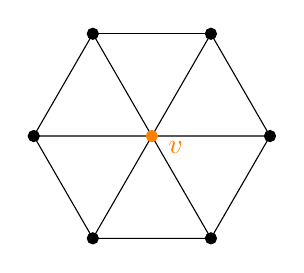
\begin{tikzpicture}
    \draw (-1.5, 0)--({-1.5*cos(60)}, {1.5*sin(60)})--(0,0)--({1.5*cos(60)}, {1.5*sin(60)})--(1.5, 0)--(0,0)--({1.5*cos(60)}, {-1.5*sin(60)})--({-1.5*cos(60)}, {-1.5*sin(60)})--(0,0)--cycle;
    \draw ({-1.5*cos(60)}, {1.5*sin(60)})--({1.5*cos(60)}, {1.5*sin(60)});
    \draw (1.5, 0)--({1.5*cos(60)}, {-1.5*sin(60)});
    \draw ({-1.5*cos(60)}, {-1.5*sin(60)})--(-1.5,0);

      %({1.5*cos(60)}, {-1.5*sin(60)})--({-1.5*cos(60)}, {-1.5*sin(60)})--cycle;
\filldraw (1.5, 0) circle (2pt);
\filldraw(-1.5, 0) circle (2pt);
\filldraw({-1.5*cos(60)}, {1.5*sin(60)}) circle (2pt);
\filldraw({1.5*cos(60)}, {1.5*sin(60)}) circle (2pt);
\filldraw({-1.5*cos(60)}, {-1.5*sin(60)}) circle (2pt);
\filldraw({1.5*cos(60)}, {-1.5*sin(60)}) circle (2pt);

\filldraw[orange](0,0) circle(2pt);
\node at (0.3, -0.15) {$\color{orange}v$};
  \end{tikzpicture}\end{center}
  Jeżeli istnieje para sąsiadów, która nie jest ze sobą połączona, to możemy pomalować je na jeden kolor. Wtedy sąsiedzi $v$ wykorzystują tylko $5$ kolorów i ostatni, szósty, pozostaje wolny do kolorowania $v$. 

  Jeśli natomiast wszyscy sąsiedzi $v$ są ze sobą połączeni, to oznacza, że mamy $K_7$ zanurzone w $G$, które z kolei jest narysowane na butelce Kleina. Wiemy, że $K_7$ nie można narysować na butelce Kleina, więc dochodzimy do sprzeczności w tym punkcie.

  To pokazuje, że przy pomocy indukcji możemy pokonać butelkę Kleina używając tylko $6$ kolorów farb.
\end{enumerate}
